\documentclass[crop,border={2pt 2pt 2pt 2pt},tikz]{standalone}
\usepackage{braket}
\usepackage{bbold}
\usepackage{bm}
\usepackage{amsmath}

\usetikzlibrary{backgrounds,decorations.markings, calc}
\tikzset{>=latex}
\tikzset{->-/.style={decoration={
  markings,
  mark=at position .55 with {\arrow{>}}},postaction={decorate}}}
\begin{document}
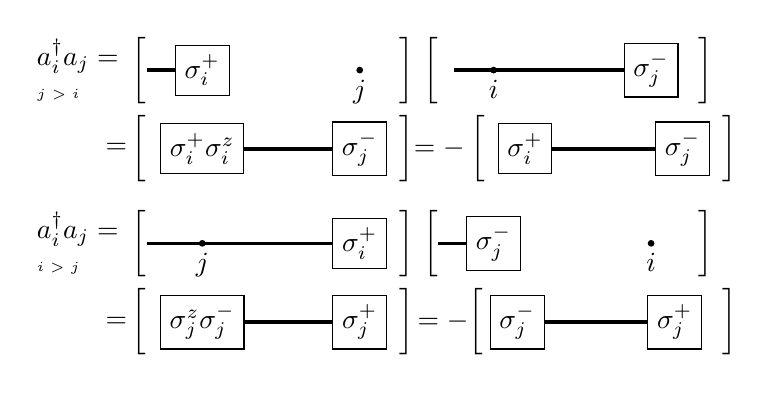
\begin{tikzpicture}[scale = 1]

    \coordinate[draw] (i) at (0,0);
    \coordinate[draw] (j) at (2,0);
    
    \node[text width =1.2cm] at ($(i) + (-1.5, 0)$) {$a^\dagger_i a_j = $ \\ {\tiny $j>i$}};
    \node[] at ($(i) + (-0.8, 0)$) {$\bigg[$};
    \draw[black,very thick] ($(i) + (-0.7,0)$) -- (i) node[draw,thin, fill = white,  anchor = center] {$\sigma^{+}_i$};
    \draw[fill, black] (j) circle (1pt) node[anchor = north] {$j$};
    \node[] at ($(j) + (0.6, 0)$) {$\bigg]$};
    
    \begin{scope}[xshift = 3.7cm ]
        \coordinate[draw] (i) at (0,0);
        \coordinate[draw] (j) at (2,0);
        
        \node[] at ($(i) + (-0.8, 0)$) {$\bigg[$};

        \draw[black,very thick] ($(j) + (-2.5,0)$) -- (j) node[draw,thin, fill = white, anchor = center] {$\sigma^{-}_j$};
        \draw[fill, black] (i) circle (1pt) node[anchor = north] {$i$};
        \node[] at ($(j) + (0.7, 0)$) {$\bigg] $}; 

        % \node[] at ($(j) + (1.5, 0)$) {$j > i$}; 

    \end{scope}

    \begin{scope}[yshift = -1cm]
        \coordinate[draw] (i) at (0,0);
        \coordinate[draw] (j) at (2,0);
        \node[] at ($(i) + (-1.5, 0)$) {$ \qquad \ = $};
        \node[] at ($(i) + (-0.8, 0)$) {$\bigg[$};
        \draw[black,very thick] (i) -- (j) node[draw,thin, fill = white, anchor = center, pos= 0] {$\sigma^{+}_i \sigma^{z}_i$} node[draw,thin, fill = white, anchor = center, pos= 1] {$\sigma^{-}_j$};
        % \draw[fill, black] (j) circle (1pt) node[anchor = north] {$j$};
        \node[] at ($(j) + (0.6, 0)$) {$\bigg]$};
    \end{scope} 

    \begin{scope}[yshift = -1cm, xshift=4.1cm]
        \coordinate[draw] (i) at (0,0);
        \coordinate[draw] (j) at (2,0);
        \node[] at ($(i) + (-1.5, 0)$) {$ \qquad \ = - $};
        \node[] at ($(i) + (-0.6, 0)$) {$\bigg[$};
        \draw[black,very thick] (i) -- (j) node[draw,thin, fill = white, anchor = center, pos= 0] {$\sigma^{+}_i$} node[draw,thin, fill = white, anchor = center, pos= 1] {$\sigma^{-}_j$};
        % \draw[fill, black] (j) circle (1pt) node[anchor = north] {$j$};
        \node[] at ($(j) + (0.6, 0)$) {$\bigg]$};
    \end{scope}
    
   
    \begin{scope}[yshift = -2.2cm]
        \coordinate[draw] (i) at (2,0);
        \coordinate[draw] (j) at (0,0);
    

        \node[text width =1.2cm] at ($(j) + (-1.5, 0)$) {$a^\dagger_i a_j = $ \\ {\tiny $i>j$}};
        \node[] at ($(j) + (-0.8, 0)$) {$\bigg[$};
        \draw[black,very thick] ($(i) + (-2.7,0)$) -- (i) node[draw,thin, fill = white, anchor = center] {$\sigma^{+}_i$};
        \draw[fill, black] (j) circle (1pt) node[anchor = north] {$j$};
        \node[] at ($(i) + (0.6, 0)$) {$\bigg]$};
    
        \begin{scope}[xshift = 3.7cm ]
            \coordinate[draw] (i) at (2,0);
            \coordinate[draw] (j) at (0,0);
            
            \node[] at ($(j) + (-0.8, 0)$) {$\bigg[$};

            \draw[black,very thick] ($(j) + (-0.7,0)$) -- (j) node[draw,thin, fill = white,  anchor = center] {$\sigma^{-}_j$};
            \draw[fill, black] (i) circle (1pt) node[anchor = north] {$i$};
            \node[] at ($(i) + (0.7, 0)$) {$\bigg] $}; 

            % \node[] at ($(i) + (1.5, 0)$) {$j < i$}; 

        \end{scope}


        \begin{scope}[yshift = -1cm]
        \coordinate[draw] (i) at (0,0);
        \coordinate[draw] (j) at (2,0);
        \node[] at ($(i) + (-1.5, 0)$) {$ \qquad \ = $};
        \node[] at ($(i) + (-0.8, 0)$) {$\bigg[$};
        \draw[black,very thick] (i) -- (j) node[draw,thin, fill = white, anchor = center, pos= 0] {$\sigma^{z}_j \sigma^{-}_j$} node[draw,thin, fill = white, anchor = center, pos= 1] {$\sigma^{+}_j$};
        % \draw[fill, black] (j) circle (1pt) node[anchor = north] {$i$};
        \node[] at ($(j) + (0.6, 0)$) {$\bigg]$};
        \begin{scope}[xshift = 4cm ]
            \coordinate[draw] (i) at (2,0);
            \coordinate[draw] (j) at (0,0);
            
            \node[] at ($(j) + (-0.85, 0)$) {$= - \bigg[$};

            \draw[black,very thick] (j) -- (i) node[draw,thin, fill = white, anchor = center, pos= 0] {$\sigma^{-}_j$} node[draw,thin, fill = white, anchor = center, pos= 1] {$\sigma^{+}_j$};
            
            \node[] at ($(i) + (0.7, 0)$) {$\bigg] $}; 

        \end{scope}
        \end{scope}
    \end{scope}

\end{tikzpicture}
\end{document}